
% Default to the notebook output style

    


% Inherit from the specified cell style.




    
\documentclass[11pt]{article}

    
    
    \usepackage[T1]{fontenc}
    % Nicer default font (+ math font) than Computer Modern for most use cases
    \usepackage{mathpazo}

    % Basic figure setup, for now with no caption control since it's done
    % automatically by Pandoc (which extracts ![](path) syntax from Markdown).
    \usepackage{graphicx}
    % We will generate all images so they have a width \maxwidth. This means
    % that they will get their normal width if they fit onto the page, but
    % are scaled down if they would overflow the margins.
    \makeatletter
    \def\maxwidth{\ifdim\Gin@nat@width>\linewidth\linewidth
    \else\Gin@nat@width\fi}
    \makeatother
    \let\Oldincludegraphics\includegraphics
    % Set max figure width to be 80% of text width, for now hardcoded.
    \renewcommand{\includegraphics}[1]{\Oldincludegraphics[width=.8\maxwidth]{#1}}
    % Ensure that by default, figures have no caption (until we provide a
    % proper Figure object with a Caption API and a way to capture that
    % in the conversion process - todo).
    \usepackage{caption}
    \DeclareCaptionLabelFormat{nolabel}{}
    \captionsetup{labelformat=nolabel}

    \usepackage{adjustbox} % Used to constrain images to a maximum size 
    \usepackage{xcolor} % Allow colors to be defined
    \usepackage{enumerate} % Needed for markdown enumerations to work
    \usepackage{geometry} % Used to adjust the document margins
    \usepackage{amsmath} % Equations
    \usepackage{amssymb} % Equations
    \usepackage{textcomp} % defines textquotesingle
    % Hack from http://tex.stackexchange.com/a/47451/13684:
    \AtBeginDocument{%
        \def\PYZsq{\textquotesingle}% Upright quotes in Pygmentized code
    }
    \usepackage{upquote} % Upright quotes for verbatim code
    \usepackage{eurosym} % defines \euro
    \usepackage[mathletters]{ucs} % Extended unicode (utf-8) support
    \usepackage[utf8x]{inputenc} % Allow utf-8 characters in the tex document
    \usepackage{fancyvrb} % verbatim replacement that allows latex
    \usepackage{grffile} % extends the file name processing of package graphics 
                         % to support a larger range 
    % The hyperref package gives us a pdf with properly built
    % internal navigation ('pdf bookmarks' for the table of contents,
    % internal cross-reference links, web links for URLs, etc.)
    \usepackage{hyperref}
    \usepackage{longtable} % longtable support required by pandoc >1.10
    \usepackage{booktabs}  % table support for pandoc > 1.12.2
    \usepackage[inline]{enumitem} % IRkernel/repr support (it uses the enumerate* environment)
    \usepackage[normalem]{ulem} % ulem is needed to support strikethroughs (\sout)
                                % normalem makes italics be italics, not underlines
    

    
    
    % Colors for the hyperref package
    \definecolor{urlcolor}{rgb}{0,.145,.698}
    \definecolor{linkcolor}{rgb}{.71,0.21,0.01}
    \definecolor{citecolor}{rgb}{.12,.54,.11}

    % ANSI colors
    \definecolor{ansi-black}{HTML}{3E424D}
    \definecolor{ansi-black-intense}{HTML}{282C36}
    \definecolor{ansi-red}{HTML}{E75C58}
    \definecolor{ansi-red-intense}{HTML}{B22B31}
    \definecolor{ansi-green}{HTML}{00A250}
    \definecolor{ansi-green-intense}{HTML}{007427}
    \definecolor{ansi-yellow}{HTML}{DDB62B}
    \definecolor{ansi-yellow-intense}{HTML}{B27D12}
    \definecolor{ansi-blue}{HTML}{208FFB}
    \definecolor{ansi-blue-intense}{HTML}{0065CA}
    \definecolor{ansi-magenta}{HTML}{D160C4}
    \definecolor{ansi-magenta-intense}{HTML}{A03196}
    \definecolor{ansi-cyan}{HTML}{60C6C8}
    \definecolor{ansi-cyan-intense}{HTML}{258F8F}
    \definecolor{ansi-white}{HTML}{C5C1B4}
    \definecolor{ansi-white-intense}{HTML}{A1A6B2}

    % commands and environments needed by pandoc snippets
    % extracted from the output of `pandoc -s`
    \providecommand{\tightlist}{%
      \setlength{\itemsep}{0pt}\setlength{\parskip}{0pt}}
    \DefineVerbatimEnvironment{Highlighting}{Verbatim}{commandchars=\\\{\}}
    % Add ',fontsize=\small' for more characters per line
    \newenvironment{Shaded}{}{}
    \newcommand{\KeywordTok}[1]{\textcolor[rgb]{0.00,0.44,0.13}{\textbf{{#1}}}}
    \newcommand{\DataTypeTok}[1]{\textcolor[rgb]{0.56,0.13,0.00}{{#1}}}
    \newcommand{\DecValTok}[1]{\textcolor[rgb]{0.25,0.63,0.44}{{#1}}}
    \newcommand{\BaseNTok}[1]{\textcolor[rgb]{0.25,0.63,0.44}{{#1}}}
    \newcommand{\FloatTok}[1]{\textcolor[rgb]{0.25,0.63,0.44}{{#1}}}
    \newcommand{\CharTok}[1]{\textcolor[rgb]{0.25,0.44,0.63}{{#1}}}
    \newcommand{\StringTok}[1]{\textcolor[rgb]{0.25,0.44,0.63}{{#1}}}
    \newcommand{\CommentTok}[1]{\textcolor[rgb]{0.38,0.63,0.69}{\textit{{#1}}}}
    \newcommand{\OtherTok}[1]{\textcolor[rgb]{0.00,0.44,0.13}{{#1}}}
    \newcommand{\AlertTok}[1]{\textcolor[rgb]{1.00,0.00,0.00}{\textbf{{#1}}}}
    \newcommand{\FunctionTok}[1]{\textcolor[rgb]{0.02,0.16,0.49}{{#1}}}
    \newcommand{\RegionMarkerTok}[1]{{#1}}
    \newcommand{\ErrorTok}[1]{\textcolor[rgb]{1.00,0.00,0.00}{\textbf{{#1}}}}
    \newcommand{\NormalTok}[1]{{#1}}
    
    % Additional commands for more recent versions of Pandoc
    \newcommand{\ConstantTok}[1]{\textcolor[rgb]{0.53,0.00,0.00}{{#1}}}
    \newcommand{\SpecialCharTok}[1]{\textcolor[rgb]{0.25,0.44,0.63}{{#1}}}
    \newcommand{\VerbatimStringTok}[1]{\textcolor[rgb]{0.25,0.44,0.63}{{#1}}}
    \newcommand{\SpecialStringTok}[1]{\textcolor[rgb]{0.73,0.40,0.53}{{#1}}}
    \newcommand{\ImportTok}[1]{{#1}}
    \newcommand{\DocumentationTok}[1]{\textcolor[rgb]{0.73,0.13,0.13}{\textit{{#1}}}}
    \newcommand{\AnnotationTok}[1]{\textcolor[rgb]{0.38,0.63,0.69}{\textbf{\textit{{#1}}}}}
    \newcommand{\CommentVarTok}[1]{\textcolor[rgb]{0.38,0.63,0.69}{\textbf{\textit{{#1}}}}}
    \newcommand{\VariableTok}[1]{\textcolor[rgb]{0.10,0.09,0.49}{{#1}}}
    \newcommand{\ControlFlowTok}[1]{\textcolor[rgb]{0.00,0.44,0.13}{\textbf{{#1}}}}
    \newcommand{\OperatorTok}[1]{\textcolor[rgb]{0.40,0.40,0.40}{{#1}}}
    \newcommand{\BuiltInTok}[1]{{#1}}
    \newcommand{\ExtensionTok}[1]{{#1}}
    \newcommand{\PreprocessorTok}[1]{\textcolor[rgb]{0.74,0.48,0.00}{{#1}}}
    \newcommand{\AttributeTok}[1]{\textcolor[rgb]{0.49,0.56,0.16}{{#1}}}
    \newcommand{\InformationTok}[1]{\textcolor[rgb]{0.38,0.63,0.69}{\textbf{\textit{{#1}}}}}
    \newcommand{\WarningTok}[1]{\textcolor[rgb]{0.38,0.63,0.69}{\textbf{\textit{{#1}}}}}
    
    
    % Define a nice break command that doesn't care if a line doesn't already
    % exist.
    \def\br{\hspace*{\fill} \\* }
    % Math Jax compatability definitions
    \def\gt{>}
    \def\lt{<}
    % Document parameters
    \title{keras-tuto}
    
    
    

    % Pygments definitions
    
\makeatletter
\def\PY@reset{\let\PY@it=\relax \let\PY@bf=\relax%
    \let\PY@ul=\relax \let\PY@tc=\relax%
    \let\PY@bc=\relax \let\PY@ff=\relax}
\def\PY@tok#1{\csname PY@tok@#1\endcsname}
\def\PY@toks#1+{\ifx\relax#1\empty\else%
    \PY@tok{#1}\expandafter\PY@toks\fi}
\def\PY@do#1{\PY@bc{\PY@tc{\PY@ul{%
    \PY@it{\PY@bf{\PY@ff{#1}}}}}}}
\def\PY#1#2{\PY@reset\PY@toks#1+\relax+\PY@do{#2}}

\expandafter\def\csname PY@tok@nn\endcsname{\let\PY@bf=\textbf\def\PY@tc##1{\textcolor[rgb]{0.00,0.00,1.00}{##1}}}
\expandafter\def\csname PY@tok@kp\endcsname{\def\PY@tc##1{\textcolor[rgb]{0.00,0.50,0.00}{##1}}}
\expandafter\def\csname PY@tok@gr\endcsname{\def\PY@tc##1{\textcolor[rgb]{1.00,0.00,0.00}{##1}}}
\expandafter\def\csname PY@tok@nb\endcsname{\def\PY@tc##1{\textcolor[rgb]{0.00,0.50,0.00}{##1}}}
\expandafter\def\csname PY@tok@ne\endcsname{\let\PY@bf=\textbf\def\PY@tc##1{\textcolor[rgb]{0.82,0.25,0.23}{##1}}}
\expandafter\def\csname PY@tok@sc\endcsname{\def\PY@tc##1{\textcolor[rgb]{0.73,0.13,0.13}{##1}}}
\expandafter\def\csname PY@tok@vc\endcsname{\def\PY@tc##1{\textcolor[rgb]{0.10,0.09,0.49}{##1}}}
\expandafter\def\csname PY@tok@nt\endcsname{\let\PY@bf=\textbf\def\PY@tc##1{\textcolor[rgb]{0.00,0.50,0.00}{##1}}}
\expandafter\def\csname PY@tok@kt\endcsname{\def\PY@tc##1{\textcolor[rgb]{0.69,0.00,0.25}{##1}}}
\expandafter\def\csname PY@tok@s\endcsname{\def\PY@tc##1{\textcolor[rgb]{0.73,0.13,0.13}{##1}}}
\expandafter\def\csname PY@tok@kd\endcsname{\let\PY@bf=\textbf\def\PY@tc##1{\textcolor[rgb]{0.00,0.50,0.00}{##1}}}
\expandafter\def\csname PY@tok@s2\endcsname{\def\PY@tc##1{\textcolor[rgb]{0.73,0.13,0.13}{##1}}}
\expandafter\def\csname PY@tok@ge\endcsname{\let\PY@it=\textit}
\expandafter\def\csname PY@tok@m\endcsname{\def\PY@tc##1{\textcolor[rgb]{0.40,0.40,0.40}{##1}}}
\expandafter\def\csname PY@tok@fm\endcsname{\def\PY@tc##1{\textcolor[rgb]{0.00,0.00,1.00}{##1}}}
\expandafter\def\csname PY@tok@ni\endcsname{\let\PY@bf=\textbf\def\PY@tc##1{\textcolor[rgb]{0.60,0.60,0.60}{##1}}}
\expandafter\def\csname PY@tok@bp\endcsname{\def\PY@tc##1{\textcolor[rgb]{0.00,0.50,0.00}{##1}}}
\expandafter\def\csname PY@tok@si\endcsname{\let\PY@bf=\textbf\def\PY@tc##1{\textcolor[rgb]{0.73,0.40,0.53}{##1}}}
\expandafter\def\csname PY@tok@mh\endcsname{\def\PY@tc##1{\textcolor[rgb]{0.40,0.40,0.40}{##1}}}
\expandafter\def\csname PY@tok@nl\endcsname{\def\PY@tc##1{\textcolor[rgb]{0.63,0.63,0.00}{##1}}}
\expandafter\def\csname PY@tok@sb\endcsname{\def\PY@tc##1{\textcolor[rgb]{0.73,0.13,0.13}{##1}}}
\expandafter\def\csname PY@tok@nf\endcsname{\def\PY@tc##1{\textcolor[rgb]{0.00,0.00,1.00}{##1}}}
\expandafter\def\csname PY@tok@nv\endcsname{\def\PY@tc##1{\textcolor[rgb]{0.10,0.09,0.49}{##1}}}
\expandafter\def\csname PY@tok@gp\endcsname{\let\PY@bf=\textbf\def\PY@tc##1{\textcolor[rgb]{0.00,0.00,0.50}{##1}}}
\expandafter\def\csname PY@tok@dl\endcsname{\def\PY@tc##1{\textcolor[rgb]{0.73,0.13,0.13}{##1}}}
\expandafter\def\csname PY@tok@gt\endcsname{\def\PY@tc##1{\textcolor[rgb]{0.00,0.27,0.87}{##1}}}
\expandafter\def\csname PY@tok@w\endcsname{\def\PY@tc##1{\textcolor[rgb]{0.73,0.73,0.73}{##1}}}
\expandafter\def\csname PY@tok@gu\endcsname{\let\PY@bf=\textbf\def\PY@tc##1{\textcolor[rgb]{0.50,0.00,0.50}{##1}}}
\expandafter\def\csname PY@tok@sd\endcsname{\let\PY@it=\textit\def\PY@tc##1{\textcolor[rgb]{0.73,0.13,0.13}{##1}}}
\expandafter\def\csname PY@tok@o\endcsname{\def\PY@tc##1{\textcolor[rgb]{0.40,0.40,0.40}{##1}}}
\expandafter\def\csname PY@tok@cp\endcsname{\def\PY@tc##1{\textcolor[rgb]{0.74,0.48,0.00}{##1}}}
\expandafter\def\csname PY@tok@cs\endcsname{\let\PY@it=\textit\def\PY@tc##1{\textcolor[rgb]{0.25,0.50,0.50}{##1}}}
\expandafter\def\csname PY@tok@vg\endcsname{\def\PY@tc##1{\textcolor[rgb]{0.10,0.09,0.49}{##1}}}
\expandafter\def\csname PY@tok@kn\endcsname{\let\PY@bf=\textbf\def\PY@tc##1{\textcolor[rgb]{0.00,0.50,0.00}{##1}}}
\expandafter\def\csname PY@tok@kr\endcsname{\let\PY@bf=\textbf\def\PY@tc##1{\textcolor[rgb]{0.00,0.50,0.00}{##1}}}
\expandafter\def\csname PY@tok@s1\endcsname{\def\PY@tc##1{\textcolor[rgb]{0.73,0.13,0.13}{##1}}}
\expandafter\def\csname PY@tok@sh\endcsname{\def\PY@tc##1{\textcolor[rgb]{0.73,0.13,0.13}{##1}}}
\expandafter\def\csname PY@tok@sr\endcsname{\def\PY@tc##1{\textcolor[rgb]{0.73,0.40,0.53}{##1}}}
\expandafter\def\csname PY@tok@mb\endcsname{\def\PY@tc##1{\textcolor[rgb]{0.40,0.40,0.40}{##1}}}
\expandafter\def\csname PY@tok@kc\endcsname{\let\PY@bf=\textbf\def\PY@tc##1{\textcolor[rgb]{0.00,0.50,0.00}{##1}}}
\expandafter\def\csname PY@tok@cpf\endcsname{\let\PY@it=\textit\def\PY@tc##1{\textcolor[rgb]{0.25,0.50,0.50}{##1}}}
\expandafter\def\csname PY@tok@go\endcsname{\def\PY@tc##1{\textcolor[rgb]{0.53,0.53,0.53}{##1}}}
\expandafter\def\csname PY@tok@ow\endcsname{\let\PY@bf=\textbf\def\PY@tc##1{\textcolor[rgb]{0.67,0.13,1.00}{##1}}}
\expandafter\def\csname PY@tok@err\endcsname{\def\PY@bc##1{\setlength{\fboxsep}{0pt}\fcolorbox[rgb]{1.00,0.00,0.00}{1,1,1}{\strut ##1}}}
\expandafter\def\csname PY@tok@gd\endcsname{\def\PY@tc##1{\textcolor[rgb]{0.63,0.00,0.00}{##1}}}
\expandafter\def\csname PY@tok@sx\endcsname{\def\PY@tc##1{\textcolor[rgb]{0.00,0.50,0.00}{##1}}}
\expandafter\def\csname PY@tok@mf\endcsname{\def\PY@tc##1{\textcolor[rgb]{0.40,0.40,0.40}{##1}}}
\expandafter\def\csname PY@tok@vi\endcsname{\def\PY@tc##1{\textcolor[rgb]{0.10,0.09,0.49}{##1}}}
\expandafter\def\csname PY@tok@ch\endcsname{\let\PY@it=\textit\def\PY@tc##1{\textcolor[rgb]{0.25,0.50,0.50}{##1}}}
\expandafter\def\csname PY@tok@k\endcsname{\let\PY@bf=\textbf\def\PY@tc##1{\textcolor[rgb]{0.00,0.50,0.00}{##1}}}
\expandafter\def\csname PY@tok@c\endcsname{\let\PY@it=\textit\def\PY@tc##1{\textcolor[rgb]{0.25,0.50,0.50}{##1}}}
\expandafter\def\csname PY@tok@gi\endcsname{\def\PY@tc##1{\textcolor[rgb]{0.00,0.63,0.00}{##1}}}
\expandafter\def\csname PY@tok@nd\endcsname{\def\PY@tc##1{\textcolor[rgb]{0.67,0.13,1.00}{##1}}}
\expandafter\def\csname PY@tok@gh\endcsname{\let\PY@bf=\textbf\def\PY@tc##1{\textcolor[rgb]{0.00,0.00,0.50}{##1}}}
\expandafter\def\csname PY@tok@cm\endcsname{\let\PY@it=\textit\def\PY@tc##1{\textcolor[rgb]{0.25,0.50,0.50}{##1}}}
\expandafter\def\csname PY@tok@il\endcsname{\def\PY@tc##1{\textcolor[rgb]{0.40,0.40,0.40}{##1}}}
\expandafter\def\csname PY@tok@no\endcsname{\def\PY@tc##1{\textcolor[rgb]{0.53,0.00,0.00}{##1}}}
\expandafter\def\csname PY@tok@gs\endcsname{\let\PY@bf=\textbf}
\expandafter\def\csname PY@tok@mi\endcsname{\def\PY@tc##1{\textcolor[rgb]{0.40,0.40,0.40}{##1}}}
\expandafter\def\csname PY@tok@sa\endcsname{\def\PY@tc##1{\textcolor[rgb]{0.73,0.13,0.13}{##1}}}
\expandafter\def\csname PY@tok@na\endcsname{\def\PY@tc##1{\textcolor[rgb]{0.49,0.56,0.16}{##1}}}
\expandafter\def\csname PY@tok@ss\endcsname{\def\PY@tc##1{\textcolor[rgb]{0.10,0.09,0.49}{##1}}}
\expandafter\def\csname PY@tok@vm\endcsname{\def\PY@tc##1{\textcolor[rgb]{0.10,0.09,0.49}{##1}}}
\expandafter\def\csname PY@tok@c1\endcsname{\let\PY@it=\textit\def\PY@tc##1{\textcolor[rgb]{0.25,0.50,0.50}{##1}}}
\expandafter\def\csname PY@tok@se\endcsname{\let\PY@bf=\textbf\def\PY@tc##1{\textcolor[rgb]{0.73,0.40,0.13}{##1}}}
\expandafter\def\csname PY@tok@mo\endcsname{\def\PY@tc##1{\textcolor[rgb]{0.40,0.40,0.40}{##1}}}
\expandafter\def\csname PY@tok@nc\endcsname{\let\PY@bf=\textbf\def\PY@tc##1{\textcolor[rgb]{0.00,0.00,1.00}{##1}}}

\def\PYZbs{\char`\\}
\def\PYZus{\char`\_}
\def\PYZob{\char`\{}
\def\PYZcb{\char`\}}
\def\PYZca{\char`\^}
\def\PYZam{\char`\&}
\def\PYZlt{\char`\<}
\def\PYZgt{\char`\>}
\def\PYZsh{\char`\#}
\def\PYZpc{\char`\%}
\def\PYZdl{\char`\$}
\def\PYZhy{\char`\-}
\def\PYZsq{\char`\'}
\def\PYZdq{\char`\"}
\def\PYZti{\char`\~}
% for compatibility with earlier versions
\def\PYZat{@}
\def\PYZlb{[}
\def\PYZrb{]}
\makeatother


    % Exact colors from NB
    \definecolor{incolor}{rgb}{0.0, 0.0, 0.5}
    \definecolor{outcolor}{rgb}{0.545, 0.0, 0.0}



    
    % Prevent overflowing lines due to hard-to-break entities
    \sloppy 
    % Setup hyperref package
    \hypersetup{
      breaklinks=true,  % so long urls are correctly broken across lines
      colorlinks=true,
      urlcolor=urlcolor,
      linkcolor=linkcolor,
      citecolor=citecolor,
      }
    % Slightly bigger margins than the latex defaults
    
    \geometry{verbose,tmargin=1in,bmargin=1in,lmargin=1in,rmargin=1in}
    
    

    \begin{document}
    
    
    \maketitle
    
    

    
    \begin{Verbatim}[commandchars=\\\{\}]
{\color{incolor}In [{\color{incolor}1}]:} \PY{c+c1}{\PYZsh{} \PYZhy{}*\PYZhy{} coding: utf\PYZhy{}8 \PYZhy{}*\PYZhy{}}
\end{Verbatim}


    \hypertarget{unhuman-project}{%
\section{Unhuman Project}\label{unhuman-project}}

    \hypertarget{tutorial---keras}{%
\subsection{Tutorial - Keras}\label{tutorial---keras}}

    In this document, I will write the python code given by the
\href{https://www.tensorflow.org/guide/keras}{TensorFlow Tutorial: Keras
Guide}

Keras is an API to help build and train artificial intelligence model,
implemented in TensorFlow library. The \emph{model} is a group of layers
which contains neurons.

    \hypertarget{get-started-with-keras}{%
\subsubsection{Get Started with Keras}\label{get-started-with-keras}}

    In Python, to import keras, the following code must be added:

    \begin{Verbatim}[commandchars=\\\{\}]
{\color{incolor}In [{\color{incolor}2}]:} \PY{k+kn}{import} \PY{n+nn}{tensorflow} \PY{k}{as} \PY{n+nn}{tf}
        \PY{k+kn}{import} \PY{n+nn}{keras}
\end{Verbatim}


    \begin{Verbatim}[commandchars=\\\{\}]
Using TensorFlow backend.

    \end{Verbatim}

    We can now use keras through \texttt{tf.keras} module.

Note that you might need to install the \texttt{keras} python package by
using:

\begin{Shaded}
\begin{Highlighting}[]
\ExtensionTok{pip}\NormalTok{ install keras}
\end{Highlighting}
\end{Shaded}

or

\begin{Shaded}
\begin{Highlighting}[]
\ExtensionTok{conda}\NormalTok{ install -n myenv keras}
\end{Highlighting}
\end{Shaded}

    \begin{Verbatim}[commandchars=\\\{\}]
{\color{incolor}In [{\color{incolor}3}]:} \PY{n+nb}{print}\PY{p}{(}\PY{l+s+s2}{\PYZdq{}}\PY{l+s+s2}{TensorFlow version: }\PY{l+s+si}{\PYZob{}0\PYZcb{}}\PY{l+s+se}{\PYZbs{}n}\PY{l+s+s2}{Keras version: }\PY{l+s+si}{\PYZob{}1\PYZcb{}}\PY{l+s+s2}{\PYZdq{}}\PY{o}{.}\PY{n}{format}\PY{p}{(}\PY{n}{tf}\PY{o}{.}\PY{n}{\PYZus{}\PYZus{}version\PYZus{}\PYZus{}}\PY{p}{,} \PY{n}{keras}\PY{o}{.}\PY{n}{\PYZus{}\PYZus{}version\PYZus{}\PYZus{}}\PY{p}{)}\PY{p}{)}
\end{Verbatim}


    \begin{Verbatim}[commandchars=\\\{\}]
TensorFlow version: 1.8.0
Keras version: 2.2.0

    \end{Verbatim}

    \hypertarget{build-simple-model}{%
\subsubsection{Build Simple Model}\label{build-simple-model}}

    \hypertarget{sequential-model}{%
\paragraph{Sequential Model}\label{sequential-model}}

    The following code build a Sequential model, with a fully-connected
neural network (multi-layer perceptron):

    \begin{Verbatim}[commandchars=\\\{\}]
{\color{incolor}In [{\color{incolor}4}]:} \PY{n}{model} \PY{o}{=} \PY{n}{tf}\PY{o}{.}\PY{n}{keras}\PY{o}{.}\PY{n}{Sequential}\PY{p}{(}\PY{p}{)}
        
        \PY{c+c1}{\PYZsh{} Add a dense layer containing 64 neurons}
        \PY{n}{model}\PY{o}{.}\PY{n}{add}\PY{p}{(}\PY{n}{tf}\PY{o}{.}\PY{n}{keras}\PY{o}{.}\PY{n}{layers}\PY{o}{.}\PY{n}{Dense}\PY{p}{(}\PY{n}{units}\PY{o}{=}\PY{l+m+mi}{64}\PY{p}{,} \PY{n}{activation}\PY{o}{=}\PY{l+s+s2}{\PYZdq{}}\PY{l+s+s2}{relu}\PY{l+s+s2}{\PYZdq{}}\PY{p}{,} \PY{n}{input\PYZus{}shape}\PY{o}{=}\PY{p}{(}\PY{l+m+mi}{32}\PY{p}{,}\PY{p}{)}\PY{p}{)}\PY{p}{)}
        
        \PY{c+c1}{\PYZsh{} Add another}
        \PY{n}{model}\PY{o}{.}\PY{n}{add}\PY{p}{(}\PY{n}{tf}\PY{o}{.}\PY{n}{keras}\PY{o}{.}\PY{n}{layers}\PY{o}{.}\PY{n}{Dense}\PY{p}{(}\PY{n}{units}\PY{o}{=}\PY{l+m+mi}{64}\PY{p}{,} \PY{n}{activation}\PY{o}{=}\PY{l+s+s2}{\PYZdq{}}\PY{l+s+s2}{relu}\PY{l+s+s2}{\PYZdq{}}\PY{p}{)}\PY{p}{)}
        
        \PY{c+c1}{\PYZsh{} Add a softmax layer with 10 output neurons}
        \PY{n}{model}\PY{o}{.}\PY{n}{add}\PY{p}{(}\PY{n}{tf}\PY{o}{.}\PY{n}{keras}\PY{o}{.}\PY{n}{layers}\PY{o}{.}\PY{n}{Dense}\PY{p}{(}\PY{n}{units}\PY{o}{=}\PY{l+m+mi}{10}\PY{p}{,} \PY{n}{activation}\PY{o}{=}\PY{l+s+s2}{\PYZdq{}}\PY{l+s+s2}{softmax}\PY{l+s+s2}{\PYZdq{}}\PY{p}{)}\PY{p}{)}
\end{Verbatim}


    As a reminder, The \texttt{relu} activation function, also called
\textbf{Rectifer function} returns 0 if the inputs \texttt{x} is less or
equal to zero, or \texttt{x} otherwise. In other words, the function
will conserve the effect during the training process. The following
formula shows the function in a more mathematical way: \begin{equation*}
f(x) = \begin{Bmatrix}
0 & if x \leq 0\\ 
x & if x > 0
\end{Bmatrix} = max(0, x)
\end{equation*} 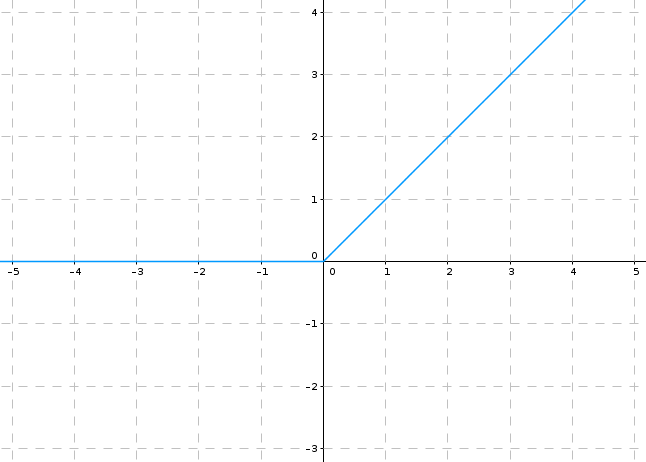
\includegraphics{../../../../../res/images/relu.png}

\begin{center}\rule{0.5\linewidth}{\linethickness}\end{center}

The \textbf{Softmax function}, on the other hand, help to train
classification model. The function \(\sigma(z)_{j}\) takes as input a
vector. The parameter \(j\) is the index of the output neuron
(\(j = 1, 2, ..., K\)). The following equation represents the Softmax
function: \begin{equation*}
\sigma(z)_{j} = \frac{e^{z_{j}}}{\sum_{k=1}^{K} e^{z_k}}
\end{equation*}

\begin{center}\rule{0.5\linewidth}{\linethickness}\end{center}

Another known activation function which is not in this python code is
\textbf{Sigmoid function}. This function is widely use in artificial
intelligence, and it is one of the most activation functions.
\begin{equation*}
f(x) = \frac{1}{1 + e^{-x}}
\end{equation*} 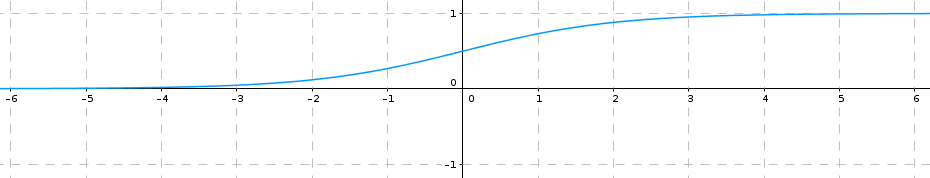
\includegraphics{../../../../../res/images/sigmoid.png}

    \hypertarget{configuration}{%
\paragraph{Configuration}\label{configuration}}

    Amongst all
\href{https://www.tensorflow.org/api_docs/python/tf/keras/layers}{\texttt{tf.keras.layers}}
constructors, there are common arguments that must be detailed before
delve into it: * \textbf{\texttt{activation=}:} The activation function
of the neurons for this specific layer. It can be a function name
(\texttt{str}) or the built-in function it-self (ex:
\texttt{tf.keras.layers.Dense(units=10,\ activation=tf.sigmoid)}). *
\textbf{\texttt{kernel\_initialize=}:} The layer's weights at
initialization, for every neuron in the layer (ex:
\texttt{kernel\_initializer="orthogonal"}). *
\textbf{\texttt{biad\_initialize=}:} The layer's bias weight only at
initialization, for every neuron in the layer (ex:
\texttt{bias\_initializer=tf.keras/initializers.constant(2.0)}). *
\textbf{\texttt{kernel\_regularizer=}:} The regularization that modify
the layer's weights (ex:
\texttt{kernel\_regularizer=tf.keras.regularizers.l1(0.01)}). By
default, there is no regularization. *
\textbf{\texttt{bias\_regularizer=}:} The regularization that modify the
layer's bias weight (ex:
\texttt{bias\_regularizer=tf.keras.regularizers.l2(0.01)}). By default,
there is no regularization.

    \hypertarget{training}{%
\subsubsection{Training}\label{training}}

    \hypertarget{configuration}{%
\paragraph{Configuration}\label{configuration}}

    The method
\href{https://www.tensorflow.org/api_docs/python/tf/keras/Model\#compile}{\texttt{tf.keras.Model.compile}}
allow the developer to configure the training process. The most relevant
arguments are: * \textbf{\texttt{optimzer=}:} The optimizer that will
train the model. See the module
\href{https://www.tensorflow.org/api_docs/python/tf/train}{\texttt{tf.train}}
for more detail, and have a look at
\href{https://www.tensorflow.org/api_docs/python/tf/train/AdamOptimizer}{\texttt{AdamOptimizer}},
\href{https://www.tensorflow.org/api_docs/python/tf/train/RMSPropOptimizer}{\texttt{RMSPropOptimizer}}
and
\href{https://www.tensorflow.org/api_docs/python/tf/train/GradientDescentOptimizer}{\texttt{GradientDescentOptimizer}}
which are the three most known optimizer in TensorFlow. *
\textbf{\texttt{loss=}:} The function that compute the error between the
computed value by the model, and the expected value (label). The code
below is the error function in the
\href{https://www.tensorflow.org/tutorials/eager/custom_training_walkthrough\#define_the_loss_and_gradient_function}{TensorFlow
eager tutorial} that can be passed as argument for this parameter:

\begin{Shaded}
\begin{Highlighting}[]
\KeywordTok{def}\NormalTok{ error(model: tf.keras.models.Model, x, y):}
    \CommentTok{"""}
\CommentTok{    Compute the error between the value returned by model(x) and the expected result y}
\CommentTok{    :param model: The model to use}
\CommentTok{    :param x: The input(s)}
\CommentTok{    :param y: The expected value that the model is supposed to return with x as input(s)}
\CommentTok{    :return: The error between the actual value and the expected value}
\CommentTok{    """}
\NormalTok{    computed_y }\OperatorTok{=}\NormalTok{ model(x)}
    \ControlFlowTok{return}\NormalTok{ tf.losses.sparse_softmax_cross_entropy(labels}\OperatorTok{=}\NormalTok{y, logits}\OperatorTok{=}\NormalTok{computed_y)}
\end{Highlighting}
\end{Shaded}

\begin{itemize}
\tightlist
\item
  \textbf{\texttt{metrics=}:} The metric to monitor and evaluate during
  the training/testing process. For more detail about this argument,
  please
  \href{https://www.tensorflow.org/api_docs/python/tf/keras/Model\#compile}{see
  the documentation about it}. This parameter accept string, list of
  string, dictionary (containing string as value) or function type
  (which are listed
  \href{https://www.tensorflow.org/api_docs/python/tf/keras/metrics}{here}).
  A typical example is \texttt{metrics={[}"accuracy"{]}} to monitor the
  accracy level, or \texttt{metrics={[}"mae"{]}} to watch the \emph{mean
  absolute error}.
\end{itemize}

For more examples about this method, please have a look at the
\href{https://www.tensorflow.org/guide/keras\#set_up_training}{TensorFlow
tutorial page}.

Now, let's configure the model:

    \begin{Verbatim}[commandchars=\\\{\}]
{\color{incolor}In [{\color{incolor}5}]:} \PY{n}{model}\PY{o}{.}\PY{n}{compile}\PY{p}{(}
            \PY{n}{optimizer}\PY{o}{=}\PY{n}{tf}\PY{o}{.}\PY{n}{train}\PY{o}{.}\PY{n}{AdamOptimizer}\PY{p}{(}\PY{l+m+mf}{0.001}\PY{p}{)}\PY{p}{,}
            \PY{n}{loss}\PY{o}{=}\PY{l+s+s2}{\PYZdq{}}\PY{l+s+s2}{categorical\PYZus{}crossentropy}\PY{l+s+s2}{\PYZdq{}}\PY{p}{,}
            \PY{n}{metrics}\PY{o}{=}\PY{p}{[}\PY{l+s+s2}{\PYZdq{}}\PY{l+s+s2}{accuracy}\PY{l+s+s2}{\PYZdq{}}\PY{p}{]}
        \PY{p}{)}
\end{Verbatim}


    \hypertarget{fit-training}{%
\paragraph{\texorpdfstring{\emph{Fit}
Training}{Fit Training}}\label{fit-training}}

    For this example, a small dataset will be used to train the model (as it
doesn't have any purpose). Fortunatly, TensorFlow has implemented a
function for that instead of passing through a training-loop. And this
alternative is
\href{https://www.tensorflow.org/api_docs/python/tf/keras/Model\#fit}{\texttt{model.fit()}}
methods, which take 5 important parameters: * \textbf{\texttt{x=}:} The
inputs (\emph{features}) (an array of array of int, for instance) *
\textbf{\texttt{y=}:} The expected outputs (\emph{labels}) *
\textbf{\texttt{batch\_size=}:} The number of \emph{slices} of inputs to
cut for each iteration. A typical value is \texttt{32}. Warning: The
last batch might be very small if the number of samples is not divisible
by \texttt{batch\_size}. * \textbf{\texttt{epochs=}:} Number of
iterations through the whole dataset input. *
\textbf{\texttt{verbose=}:} (\emph{Optional}) Set the log level: 0 for
quiet mode, 1 to display a progressbar (default), or 2 for one line per
epoch. * \textbf{\texttt{validation\_data=}:} (\emph{Optional}) Tuple of
features and labels. The \texttt{fit} function will compute the error
made by the model at each iteration using this dataset and print it.

Time for training the model. I will use the library
\href{https://www.numpy.org/}{NumPy} to generate a random dataset:

    \begin{Verbatim}[commandchars=\\\{\}]
{\color{incolor}In [{\color{incolor}6}]:} \PY{k+kn}{import} \PY{n+nn}{numpy} \PY{k}{as} \PY{n+nn}{np}
        
        \PY{n}{features} \PY{o}{=} \PY{n}{np}\PY{o}{.}\PY{n}{random}\PY{o}{.}\PY{n}{random}\PY{p}{(}\PY{p}{(}\PY{l+m+mi}{1000}\PY{p}{,} \PY{l+m+mi}{32}\PY{p}{)}\PY{p}{)} \PY{c+c1}{\PYZsh{} Generate an array containing 1000 array which contain 32 values each}
        \PY{n}{labels}   \PY{o}{=} \PY{n}{np}\PY{o}{.}\PY{n}{random}\PY{o}{.}\PY{n}{random}\PY{p}{(}\PY{p}{(}\PY{l+m+mi}{1000}\PY{p}{,} \PY{l+m+mi}{10}\PY{p}{)}\PY{p}{)} \PY{c+c1}{\PYZsh{} array containing 1000 arrays containing 10 values}
        
        \PY{n}{val\PYZus{}features} \PY{o}{=} \PY{n}{np}\PY{o}{.}\PY{n}{random}\PY{o}{.}\PY{n}{random}\PY{p}{(}\PY{p}{(}\PY{l+m+mi}{1000}\PY{p}{,} \PY{l+m+mi}{32}\PY{p}{)}\PY{p}{)}
        \PY{n}{val\PYZus{}labels}   \PY{o}{=} \PY{n}{np}\PY{o}{.}\PY{n}{random}\PY{o}{.}\PY{n}{random}\PY{p}{(}\PY{p}{(}\PY{l+m+mi}{1000}\PY{p}{,} \PY{l+m+mi}{10}\PY{p}{)}\PY{p}{)}
        
        \PY{n}{model}\PY{o}{.}\PY{n}{fit}\PY{p}{(}
            \PY{n}{x}\PY{o}{=}\PY{n}{features}\PY{p}{,}
            \PY{n}{y}\PY{o}{=}\PY{n}{labels}\PY{p}{,}
            \PY{n}{batch\PYZus{}size}\PY{o}{=}\PY{l+m+mi}{32}\PY{p}{,}
            \PY{n}{epochs}\PY{o}{=}\PY{l+m+mi}{10}\PY{p}{,}
            \PY{n}{validation\PYZus{}data}\PY{o}{=}\PY{p}{(}\PY{n}{val\PYZus{}features}\PY{p}{,} \PY{n}{val\PYZus{}labels}\PY{p}{)}
        \PY{p}{)}
\end{Verbatim}


    \begin{Verbatim}[commandchars=\\\{\}]
Train on 1000 samples, validate on 1000 samples
Epoch 1/10
1000/1000 [==============================] - 0s 361us/step - loss: 11.6062 - acc: 0.1080 - val\_loss: 11.6737 - val\_acc: 0.1100
Epoch 2/10
1000/1000 [==============================] - 0s 119us/step - loss: 11.5608 - acc: 0.1360 - val\_loss: 11.6673 - val\_acc: 0.1110
Epoch 3/10
1000/1000 [==============================] - 0s 117us/step - loss: 11.5542 - acc: 0.1290 - val\_loss: 11.6651 - val\_acc: 0.1120
Epoch 4/10
1000/1000 [==============================] - 0s 115us/step - loss: 11.5489 - acc: 0.1380 - val\_loss: 11.6654 - val\_acc: 0.1060
Epoch 5/10
1000/1000 [==============================] - 0s 123us/step - loss: 11.5435 - acc: 0.1490 - val\_loss: 11.6652 - val\_acc: 0.1120
Epoch 6/10
1000/1000 [==============================] - 0s 114us/step - loss: 11.5414 - acc: 0.1450 - val\_loss: 11.6660 - val\_acc: 0.1210
Epoch 7/10
1000/1000 [==============================] - 0s 115us/step - loss: 11.5366 - acc: 0.1630 - val\_loss: 11.6657 - val\_acc: 0.1180
Epoch 8/10
1000/1000 [==============================] - 0s 126us/step - loss: 11.5329 - acc: 0.1500 - val\_loss: 11.6658 - val\_acc: 0.1070
Epoch 9/10
1000/1000 [==============================] - 0s 115us/step - loss: 11.5280 - acc: 0.1640 - val\_loss: 11.6693 - val\_acc: 0.1070
Epoch 10/10
1000/1000 [==============================] - 0s 116us/step - loss: 11.5235 - acc: 0.1610 - val\_loss: 11.6720 - val\_acc: 0.1150

    \end{Verbatim}

\begin{Verbatim}[commandchars=\\\{\}]
{\color{outcolor}Out[{\color{outcolor}6}]:} <tensorflow.python.keras.\_impl.keras.callbacks.History at 0x7ff41bf03048>
\end{Verbatim}
            
    If you execute this code, you must see above the output given by the
\texttt{fit} function after computing the validation data at each
iteration. You may found a very high loss value (\textasciitilde{}11.5)
and an accuracy value very low (\textasciitilde{}0.1). The answer of
this paradox is that the training dataset and the validation dataset are
both \textbf{randomly generated}, and then they might not have any link
between those two sets. So don't worry if you find such values.

Now let's see how to train the model with larger dataset. In this case,
the \texttt{fit} function must take the class
\href{https://www.tensorflow.org/api_docs/python/tf/data/Dataset}{\texttt{tf.data.Dataset}}.
For more information about the Dataset class, please see the
\href{https://www.tensorflow.org/guide/datasets}{tutorial related to
that subject}. An additional argument is required for this case:
\textbf{\texttt{steps\_per\_epoch}} take an integer that will set the
number of training step to run before moving to the next iteration.
Finally, as \texttt{Dataset} is a TensorFlow-type, there is no need to
specify the batch as it is wrapped in the \texttt{Dataset} instance:

    \begin{Verbatim}[commandchars=\\\{\}]
{\color{incolor}In [{\color{incolor}7}]:} \PY{n}{dataset} \PY{o}{=} \PY{n}{tf}\PY{o}{.}\PY{n}{data}\PY{o}{.}\PY{n}{Dataset}\PY{o}{.}\PY{n}{from\PYZus{}tensor\PYZus{}slices}\PY{p}{(}\PY{p}{(}\PY{n}{features}\PY{p}{,} \PY{n}{labels}\PY{p}{)}\PY{p}{)}
        \PY{n}{dataset} \PY{o}{=} \PY{n}{dataset}\PY{o}{.}\PY{n}{batch}\PY{p}{(}\PY{l+m+mi}{32}\PY{p}{)}\PY{o}{.}\PY{n}{repeat}\PY{p}{(}\PY{p}{)}
        
        \PY{n}{val\PYZus{}dataset} \PY{o}{=} \PY{n}{tf}\PY{o}{.}\PY{n}{data}\PY{o}{.}\PY{n}{Dataset}\PY{o}{.}\PY{n}{from\PYZus{}tensor\PYZus{}slices}\PY{p}{(}\PY{p}{(}\PY{n}{val\PYZus{}features}\PY{p}{,} \PY{n}{val\PYZus{}labels}\PY{p}{)}\PY{p}{)}
        \PY{n}{val\PYZus{}dataset} \PY{o}{=} \PY{n}{val\PYZus{}dataset}\PY{o}{.}\PY{n}{batch}\PY{p}{(}\PY{l+m+mi}{32}\PY{p}{)}\PY{o}{.}\PY{n}{repeat}\PY{p}{(}\PY{p}{)}
        
        \PY{k+kn}{import} \PY{n+nn}{logging}
        
        \PY{k}{try}\PY{p}{:}
            \PY{n}{model}\PY{o}{.}\PY{n}{fit}\PY{p}{(}
                \PY{n}{x}\PY{o}{=}\PY{n}{dataset}\PY{p}{,}
                \PY{n}{epochs}\PY{o}{=}\PY{l+m+mi}{10}\PY{p}{,}
                \PY{n}{steps\PYZus{}per\PYZus{}epoch}\PY{o}{=}\PY{l+m+mi}{30}\PY{p}{,}
                \PY{n}{validation\PYZus{}data}\PY{o}{=}\PY{n}{val\PYZus{}dataset}\PY{p}{,}
                \PY{n}{validation\PYZus{}steps}\PY{o}{=}\PY{l+m+mi}{3}
            \PY{p}{)}
        \PY{k}{except} \PY{p}{(}\PY{n+ne}{ValueError}\PY{p}{,} \PY{n+ne}{AttributeError}\PY{p}{)} \PY{k}{as} \PY{n}{e}\PY{p}{:}
            \PY{n}{logging}\PY{o}{.}\PY{n}{exception}\PY{p}{(}\PY{l+s+s2}{\PYZdq{}}\PY{l+s+s2}{Error while training model}\PY{l+s+s2}{\PYZdq{}}\PY{p}{)}
\end{Verbatim}


    \begin{Verbatim}[commandchars=\\\{\}]
ERROR:root:Error while training model
Traceback (most recent call last):
  File "<ipython-input-7-d90b06a579a9>", line 15, in <module>
    validation\_steps=3
  File "/home/valentin/anaconda3/envs/tensorflow/lib/python3.5/site-packages/tensorflow/python/keras/\_impl/keras/engine/training.py", line 1143, in fit
    batch\_size=batch\_size)
  File "/home/valentin/anaconda3/envs/tensorflow/lib/python3.5/site-packages/tensorflow/python/keras/\_impl/keras/engine/training.py", line 765, in \_standardize\_user\_data
    exception\_prefix='input')
  File "/home/valentin/anaconda3/envs/tensorflow/lib/python3.5/site-packages/tensorflow/python/keras/\_impl/keras/engine/training\_utils.py", line 150, in standardize\_input\_data
    data = [standardize\_single\_array(x) for x in data]
  File "/home/valentin/anaconda3/envs/tensorflow/lib/python3.5/site-packages/tensorflow/python/keras/\_impl/keras/engine/training\_utils.py", line 150, in <listcomp>
    data = [standardize\_single\_array(x) for x in data]
  File "/home/valentin/anaconda3/envs/tensorflow/lib/python3.5/site-packages/tensorflow/python/keras/\_impl/keras/engine/training\_utils.py", line 88, in standardize\_single\_array
    elif x.ndim == 1:
AttributeError: 'RepeatDataset' object has no attribute 'ndim'

    \end{Verbatim}

    \hypertarget{evaluation-prediction}{%
\paragraph{Evaluation \& Prediction}\label{evaluation-prediction}}

    This is it! The model is finally ready to evaluate and predict some
stuff! For that, the methods
\href{https://www.tensorflow.org/api_docs/python/tf/keras/Model\#evaluate}{\texttt{model.evaluate()}}
and
\href{https://www.tensorflow.org/api_docs/python/tf/keras/Model\#predict}{\texttt{model.predict()}}
will be used.

The evaluation test the model by taking \emph{features} and
\emph{labels} as argument, and print the accuracy of the artificial
intelligence:

    \begin{Verbatim}[commandchars=\\\{\}]
{\color{incolor}In [{\color{incolor}8}]:} \PY{c+c1}{\PYZsh{} Use same dataset as for training}
        \PY{n+nb}{print}\PY{p}{(}\PY{n}{model}\PY{o}{.}\PY{n}{evaluate}\PY{p}{(}\PY{n}{features}\PY{p}{,} \PY{n}{labels}\PY{p}{,} \PY{n}{batch\PYZus{}size}\PY{o}{=}\PY{l+m+mi}{32}\PY{p}{)}\PY{p}{)}
        
        \PY{k}{try}\PY{p}{:}
            \PY{n}{model}\PY{o}{.}\PY{n}{evaluate}\PY{p}{(}\PY{n}{dataset}\PY{p}{,} \PY{n}{steps}\PY{o}{=}\PY{l+m+mi}{30}\PY{p}{)}
        \PY{k}{except} \PY{n+ne}{AttributeError}\PY{p}{:}
            \PY{k}{pass}
        
        \PY{c+c1}{\PYZsh{} Use new dataset}
        \PY{n}{eval\PYZus{}features} \PY{o}{=} \PY{n}{np}\PY{o}{.}\PY{n}{random}\PY{o}{.}\PY{n}{random}\PY{p}{(}\PY{p}{(}\PY{l+m+mi}{1000}\PY{p}{,} \PY{l+m+mi}{32}\PY{p}{)}\PY{p}{)}
        \PY{n}{eval\PYZus{}labels}   \PY{o}{=} \PY{n}{np}\PY{o}{.}\PY{n}{random}\PY{o}{.}\PY{n}{random}\PY{p}{(}\PY{p}{(}\PY{l+m+mi}{1000}\PY{p}{,} \PY{l+m+mi}{10}\PY{p}{)}\PY{p}{)}
        
        \PY{n+nb}{print}\PY{p}{(}\PY{n}{model}\PY{o}{.}\PY{n}{evaluate}\PY{p}{(}\PY{n}{eval\PYZus{}features}\PY{p}{,} \PY{n}{eval\PYZus{}labels}\PY{p}{,} \PY{n}{batch\PYZus{}size}\PY{o}{=}\PY{l+m+mi}{32}\PY{p}{)}\PY{p}{)}
\end{Verbatim}


    \begin{Verbatim}[commandchars=\\\{\}]
1000/1000 [==============================] - 0s 56us/step
[11.518468627929687, 0.18]
1000/1000 [==============================] - 0s 42us/step
[11.534138961791992, 0.092]

    \end{Verbatim}

    Again, the loss and accuracy values show that the model is not
well-trained (because of the randomly-generated datasets)

Now, let's see the model making predictions:

    \begin{Verbatim}[commandchars=\\\{\}]
{\color{incolor}In [{\color{incolor}9}]:} \PY{n+nb}{print}\PY{p}{(}\PY{n}{model}\PY{o}{.}\PY{n}{predict}\PY{p}{(}\PY{n}{features}\PY{p}{,} \PY{n}{batch\PYZus{}size}\PY{o}{=}\PY{l+m+mi}{32}\PY{p}{)}\PY{p}{)}
        \PY{n+nb}{print}\PY{p}{(}\PY{n}{model}\PY{o}{.}\PY{n}{predict}\PY{p}{(}\PY{n}{np}\PY{o}{.}\PY{n}{random}\PY{o}{.}\PY{n}{random}\PY{p}{(}\PY{p}{(}\PY{l+m+mi}{1}\PY{p}{,} \PY{l+m+mi}{32}\PY{p}{)}\PY{p}{)}\PY{p}{,} \PY{n}{batch\PYZus{}size}\PY{o}{=}\PY{l+m+mi}{32}\PY{p}{)}\PY{p}{)}
        
        \PY{k}{try}\PY{p}{:}
            \PY{n}{model}\PY{o}{.}\PY{n}{predict}\PY{p}{(}\PY{n}{dataset}\PY{p}{,} \PY{n}{steps}\PY{o}{=}\PY{l+m+mi}{30}\PY{p}{)}
        \PY{k}{except} \PY{n+ne}{AttributeError}\PY{p}{:}
            \PY{k}{pass}
\end{Verbatim}


    \begin{Verbatim}[commandchars=\\\{\}]
[[0.10081632 0.08979782 0.10821775 {\ldots} 0.09983447 0.08404636 0.1023262 ]
 [0.10339455 0.09912369 0.12255173 {\ldots} 0.0937908  0.10739163 0.08710605]
 [0.10187528 0.09521687 0.0908919  {\ldots} 0.11371332 0.11051942 0.12059256]
 {\ldots}
 [0.09893441 0.08792576 0.10263261 {\ldots} 0.11127504 0.10023952 0.09765314]
 [0.09226058 0.11307584 0.10389612 {\ldots} 0.0930002  0.08187059 0.07726819]
 [0.10020598 0.08490692 0.09605562 {\ldots} 0.10818541 0.09420434 0.09171209]]
[[0.10090259 0.11700641 0.10181001 0.09832995 0.0956001  0.09510119
  0.09034132 0.10304337 0.10387025 0.09399482]]

    \end{Verbatim}

    \hypertarget{advanced-model}{%
\subsubsection{Advanced Model}\label{advanced-model}}

    The
\href{https://www.tensorflow.org/api_docs/python/tf/keras/Sequential}{\texttt{tf.keras.Sequential}}
class to generate a model is cute, but not very effective all the time.
Depending on the problem, other type of model might be selected (for
more information about Keras model, see the
\href{https://keras.io/getting-started/functional-api-guide/}{functional
API guide})

    \hypertarget{save-load}{%
\subsubsection{Save \& Load}\label{save-load}}

    \hypertarget{weights}{%
\paragraph{Weights}\label{weights}}

    From now on, we created a model, train it, evaluate it, to finally make
prediction. But imagine now that the training is an incredibly long
process (this is the case in the real world), same for the evaluation
phase. Do you believe that each time your computer or your server will
train it from scratch at every startup? Of course, it would be a waste
of time. Fortunatly for us, TensorFlow developers implemented a way to
save and restore our model. In this example, my model will be saved in
this folder:

    \begin{Verbatim}[commandchars=\\\{\}]
{\color{incolor}In [{\color{incolor}10}]:} \PY{n}{model\PYZus{}path} \PY{o}{=} \PY{l+s+s2}{\PYZdq{}}\PY{l+s+s2}{../../../../../res/saved\PYZus{}models/keras\PYZus{}tuto\PYZus{}model}\PY{l+s+s2}{\PYZdq{}}
\end{Verbatim}


    The TensorFlow team created the method
\href{https://www.tensorflow.org/api_docs/python/tf/keras/Model\#save_weights}{\texttt{model.save\_weights()}}
to save the model weights, so you only have to run the training process
once. Then, you can call
\href{https://www.tensorflow.org/api_docs/python/tf/keras/Model\#load_weights}{\texttt{model.load\_weights()}}
to load your model every time you need to! Ideally, a small evaluation
would be perfect to assess the loaded model. The code below described
this very simple in only 3 lines of code:

    \begin{Verbatim}[commandchars=\\\{\}]
{\color{incolor}In [{\color{incolor}11}]:} \PY{k+kn}{import} \PY{n+nn}{h5py}
         
         \PY{n}{model}\PY{o}{.}\PY{n}{save\PYZus{}weights}\PY{p}{(}\PY{n}{model\PYZus{}path} \PY{o}{+} \PY{l+s+s2}{\PYZdq{}}\PY{l+s+s2}{\PYZus{}weights}\PY{l+s+s2}{\PYZdq{}}\PY{p}{)}
         \PY{n}{model}\PY{o}{.}\PY{n}{load\PYZus{}weights}\PY{p}{(}\PY{n}{model\PYZus{}path} \PY{o}{+} \PY{l+s+s2}{\PYZdq{}}\PY{l+s+s2}{\PYZus{}weights}\PY{l+s+s2}{\PYZdq{}}\PY{p}{)}
\end{Verbatim}


    You may have see that the python package h5py is required. If you are on
Debian/Ubuntu, you must run the following command:

\begin{Shaded}
\begin{Highlighting}[]
\FunctionTok{sudo}\NormalTok{ apt-get install libhdf5-dev}
\end{Highlighting}
\end{Shaded}

Then, the python package h5py must be installed in your environment. If
you use pip, you can run this command:

\begin{Shaded}
\begin{Highlighting}[]
\ExtensionTok{pip}\NormalTok{ install h5py}
\end{Highlighting}
\end{Shaded}

If you use an Anaconda environment, run that command:

\begin{Shaded}
\begin{Highlighting}[]
\ExtensionTok{conda}\NormalTok{ install -n myenv h5py}
\end{Highlighting}
\end{Shaded}

Please the the
\href{https://stackoverflow.com/questions/43385565/importerrorsave-weights-requires-h5py}{Stack
Overflow forum about this subject for more details}.

The file created is a
\href{https://www.tensorflow.org/guide/checkpoints}{TensorFlow
checkpoint file}, but we can specify to save our model according to the
Keras HDF5 file format:

    \begin{Verbatim}[commandchars=\\\{\}]
{\color{incolor}In [{\color{incolor}12}]:} \PY{k}{try}\PY{p}{:}
             \PY{n}{model}\PY{o}{.}\PY{n}{save\PYZus{}weights}\PY{p}{(}\PY{n}{model\PYZus{}path} \PY{o}{+} \PY{l+s+s2}{\PYZdq{}}\PY{l+s+s2}{\PYZus{}weights.h5}\PY{l+s+s2}{\PYZdq{}}\PY{p}{,} \PY{n}{save\PYZus{}format}\PY{o}{=}\PY{l+s+s2}{\PYZdq{}}\PY{l+s+s2}{h5}\PY{l+s+s2}{\PYZdq{}}\PY{p}{)}
             \PY{n}{model}\PY{o}{.}\PY{n}{load\PYZus{}weights}\PY{p}{(}\PY{n}{model\PYZus{}path} \PY{o}{+} \PY{l+s+s2}{\PYZdq{}}\PY{l+s+s2}{\PYZus{}weights.h5}\PY{l+s+s2}{\PYZdq{}}\PY{p}{)}
         \PY{k}{except} \PY{n+ne}{TypeError}\PY{p}{:}
             \PY{n}{logging}\PY{o}{.}\PY{n}{exception}\PY{p}{(}\PY{l+s+s2}{\PYZdq{}}\PY{l+s+s2}{Error while saving|loading model}\PY{l+s+s2}{\PYZdq{}}\PY{p}{)}
\end{Verbatim}


    \begin{Verbatim}[commandchars=\\\{\}]
ERROR:root:Error while saving|loading model
Traceback (most recent call last):
  File "<ipython-input-12-92659b39e074>", line 2, in <module>
    model.save\_weights(model\_path + "\_weights.h5", save\_format="h5")
TypeError: save\_weights() got an unexpected keyword argument 'save\_format'

    \end{Verbatim}

    \hypertarget{configuration}{%
\paragraph{Configuration}\label{configuration}}

    Previously, we saved only the \textbf{weights} of the model, but now we
will save the configuration only as a JSON or YAML format:

    \begin{Verbatim}[commandchars=\\\{\}]
{\color{incolor}In [{\color{incolor}13}]:} \PY{c+c1}{\PYZsh{} Get the JSON string format of the model:}
         \PY{n}{json\PYZus{}format} \PY{o}{=} \PY{n}{model}\PY{o}{.}\PY{n}{to\PYZus{}json}\PY{p}{(}\PY{p}{)}
         \PY{n+nb}{print}\PY{p}{(}\PY{n}{json\PYZus{}format}\PY{p}{)}
         
         \PY{c+c1}{\PYZsh{} Write it}
         \PY{k}{with} \PY{n+nb}{open}\PY{p}{(}\PY{n}{model\PYZus{}path} \PY{o}{+} \PY{l+s+s2}{\PYZdq{}}\PY{l+s+s2}{\PYZus{}config.json}\PY{l+s+s2}{\PYZdq{}}\PY{p}{,} \PY{l+s+s1}{\PYZsq{}}\PY{l+s+s1}{w}\PY{l+s+s1}{\PYZsq{}}\PY{p}{)} \PY{k}{as} \PY{n}{f}\PY{p}{:}
             \PY{n}{f}\PY{o}{.}\PY{n}{write}\PY{p}{(}\PY{n}{json\PYZus{}format} \PY{o}{+} \PY{l+s+s2}{\PYZdq{}}\PY{l+s+se}{\PYZbs{}n}\PY{l+s+s2}{\PYZdq{}}\PY{p}{)}
         
         \PY{k}{del} \PY{n}{json\PYZus{}format}
         
         \PY{c+c1}{\PYZsh{} Read it}
         \PY{n}{json\PYZus{}format} \PY{o}{=} \PY{k+kc}{None}
         \PY{k}{with} \PY{n+nb}{open}\PY{p}{(}\PY{n}{model\PYZus{}path} \PY{o}{+} \PY{l+s+s2}{\PYZdq{}}\PY{l+s+s2}{\PYZus{}config.json}\PY{l+s+s2}{\PYZdq{}}\PY{p}{,} \PY{l+s+s1}{\PYZsq{}}\PY{l+s+s1}{r}\PY{l+s+s1}{\PYZsq{}}\PY{p}{)} \PY{k}{as} \PY{n}{f}\PY{p}{:}
             \PY{n}{json\PYZus{}format} \PY{o}{=} \PY{n}{f}\PY{o}{.}\PY{n}{read}\PY{p}{(}\PY{p}{)}
         
         \PY{k}{assert} \PY{n}{json\PYZus{}format} \PY{o}{!=} \PY{k+kc}{None}
         
         \PY{n}{new\PYZus{}model} \PY{o}{=} \PY{n}{keras}\PY{o}{.}\PY{n}{models}\PY{o}{.}\PY{n}{model\PYZus{}from\PYZus{}json}\PY{p}{(}\PY{n}{json\PYZus{}format}\PY{p}{)}
\end{Verbatim}


    \begin{Verbatim}[commandchars=\\\{\}]
\{"config": [\{"config": \{"trainable": true, "activation": "relu", "use\_bias": true, "dtype": "float32", "kernel\_constraint": null, "bias\_initializer": \{"config": \{"dtype": "float32"\}, "class\_name": "Zeros"\}, "name": "dense\_1", "bias\_regularizer": null, "batch\_input\_shape": [null, 32], "activity\_regularizer": null, "units": 64, "bias\_constraint": null, "kernel\_regularizer": null, "kernel\_initializer": \{"config": \{"dtype": "float32", "scale": 1.0, "mode": "fan\_avg", "seed": null, "distribution": "uniform"\}, "class\_name": "VarianceScaling"\}\}, "class\_name": "Dense"\}, \{"config": \{"dtype": "float32", "activation": "relu", "use\_bias": true, "bias\_constraint": null, "kernel\_constraint": null, "bias\_initializer": \{"config": \{"dtype": "float32"\}, "class\_name": "Zeros"\}, "name": "dense\_2", "bias\_regularizer": null, "activity\_regularizer": null, "units": 64, "trainable": true, "kernel\_regularizer": null, "kernel\_initializer": \{"config": \{"dtype": "float32", "scale": 1.0, "mode": "fan\_avg", "seed": null, "distribution": "uniform"\}, "class\_name": "VarianceScaling"\}\}, "class\_name": "Dense"\}, \{"config": \{"dtype": "float32", "activation": "softmax", "use\_bias": true, "bias\_constraint": null, "kernel\_constraint": null, "bias\_initializer": \{"config": \{"dtype": "float32"\}, "class\_name": "Zeros"\}, "name": "dense\_3", "bias\_regularizer": null, "activity\_regularizer": null, "units": 10, "trainable": true, "kernel\_regularizer": null, "kernel\_initializer": \{"config": \{"dtype": "float32", "scale": 1.0, "mode": "fan\_avg", "seed": null, "distribution": "uniform"\}, "class\_name": "VarianceScaling"\}\}, "class\_name": "Dense"\}], "keras\_version": "2.1.5-tf", "backend": "tensorflow", "class\_name": "Sequential"\}

    \end{Verbatim}

    Now, let's serialize the model in YAML:

    \begin{Verbatim}[commandchars=\\\{\}]
{\color{incolor}In [{\color{incolor}14}]:} \PY{c+c1}{\PYZsh{} Get the YAML string format of the model:}
         \PY{n}{yaml\PYZus{}format} \PY{o}{=} \PY{n}{model}\PY{o}{.}\PY{n}{to\PYZus{}yaml}\PY{p}{(}\PY{p}{)}
         \PY{n+nb}{print}\PY{p}{(}\PY{n}{yaml\PYZus{}format}\PY{p}{)}
         
         \PY{c+c1}{\PYZsh{} Write it}
         \PY{k}{with} \PY{n+nb}{open}\PY{p}{(}\PY{n}{model\PYZus{}path} \PY{o}{+} \PY{l+s+s2}{\PYZdq{}}\PY{l+s+s2}{\PYZus{}config.yaml}\PY{l+s+s2}{\PYZdq{}}\PY{p}{,} \PY{l+s+s1}{\PYZsq{}}\PY{l+s+s1}{w}\PY{l+s+s1}{\PYZsq{}}\PY{p}{)} \PY{k}{as} \PY{n}{f}\PY{p}{:}
             \PY{n}{f}\PY{o}{.}\PY{n}{write}\PY{p}{(}\PY{n}{yaml\PYZus{}format} \PY{o}{+} \PY{l+s+s2}{\PYZdq{}}\PY{l+s+se}{\PYZbs{}n}\PY{l+s+s2}{\PYZdq{}}\PY{p}{)}
         
         \PY{k}{del} \PY{n}{yaml\PYZus{}format}
         
         \PY{c+c1}{\PYZsh{} Read it}
         \PY{n}{yaml\PYZus{}format} \PY{o}{=} \PY{k+kc}{None}
         \PY{k}{with} \PY{n+nb}{open}\PY{p}{(}\PY{n}{model\PYZus{}path} \PY{o}{+} \PY{l+s+s2}{\PYZdq{}}\PY{l+s+s2}{\PYZus{}config.yaml}\PY{l+s+s2}{\PYZdq{}}\PY{p}{,} \PY{l+s+s1}{\PYZsq{}}\PY{l+s+s1}{r}\PY{l+s+s1}{\PYZsq{}}\PY{p}{)} \PY{k}{as} \PY{n}{f}\PY{p}{:}
             \PY{n}{yaml\PYZus{}format} \PY{o}{=} \PY{n}{f}\PY{o}{.}\PY{n}{read}\PY{p}{(}\PY{p}{)}
         
         \PY{k}{assert} \PY{n}{yaml\PYZus{}format} \PY{o}{!=} \PY{k+kc}{None}
         
         \PY{n}{new\PYZus{}model} \PY{o}{=} \PY{n}{keras}\PY{o}{.}\PY{n}{models}\PY{o}{.}\PY{n}{model\PYZus{}from\PYZus{}yaml}\PY{p}{(}\PY{n}{yaml\PYZus{}format}\PY{p}{)}
\end{Verbatim}


    \begin{Verbatim}[commandchars=\\\{\}]
backend: tensorflow
class\_name: Sequential
config:
- class\_name: Dense
  config:
    activation: relu
    activity\_regularizer: null
    batch\_input\_shape: !!python/tuple [null, 32]
    bias\_constraint: null
    bias\_initializer:
      class\_name: Zeros
      config: \{dtype: float32\}
    bias\_regularizer: null
    dtype: float32
    kernel\_constraint: null
    kernel\_initializer:
      class\_name: VarianceScaling
      config: \{distribution: uniform, dtype: float32, mode: fan\_avg, scale: 1.0, seed: null\}
    kernel\_regularizer: null
    name: dense\_1
    trainable: true
    units: 64
    use\_bias: true
- class\_name: Dense
  config:
    activation: relu
    activity\_regularizer: null
    bias\_constraint: null
    bias\_initializer:
      class\_name: Zeros
      config: \{dtype: float32\}
    bias\_regularizer: null
    dtype: float32
    kernel\_constraint: null
    kernel\_initializer:
      class\_name: VarianceScaling
      config: \{distribution: uniform, dtype: float32, mode: fan\_avg, scale: 1.0, seed: null\}
    kernel\_regularizer: null
    name: dense\_2
    trainable: true
    units: 64
    use\_bias: true
- class\_name: Dense
  config:
    activation: softmax
    activity\_regularizer: null
    bias\_constraint: null
    bias\_initializer:
      class\_name: Zeros
      config: \{dtype: float32\}
    bias\_regularizer: null
    dtype: float32
    kernel\_constraint: null
    kernel\_initializer:
      class\_name: VarianceScaling
      config: \{distribution: uniform, dtype: float32, mode: fan\_avg, scale: 1.0, seed: null\}
    kernel\_regularizer: null
    name: dense\_3
    trainable: true
    units: 10
    use\_bias: true
keras\_version: 2.1.5-tf


    \end{Verbatim}

    \hypertarget{entire-model}{%
\paragraph{Entire model}\label{entire-model}}

    In most of the case, you will save the \textbf{entire model}, including
the \textbf{weights}, the \textbf{configuration} and the
\textbf{optimizer}:

    \begin{Verbatim}[commandchars=\\\{\}]
{\color{incolor}In [{\color{incolor}15}]:} \PY{n}{model} \PY{o}{=} \PY{n}{tf}\PY{o}{.}\PY{n}{keras}\PY{o}{.}\PY{n}{Sequential}\PY{p}{(}\PY{p}{)}
         \PY{n}{model}\PY{o}{.}\PY{n}{add}\PY{p}{(}\PY{n}{tf}\PY{o}{.}\PY{n}{keras}\PY{o}{.}\PY{n}{layers}\PY{o}{.}\PY{n}{Dense}\PY{p}{(}\PY{n}{units}\PY{o}{=}\PY{l+m+mi}{64}\PY{p}{,} \PY{n}{activation}\PY{o}{=}\PY{l+s+s2}{\PYZdq{}}\PY{l+s+s2}{relu}\PY{l+s+s2}{\PYZdq{}}\PY{p}{,} \PY{n}{input\PYZus{}shape}\PY{o}{=}\PY{p}{(}\PY{l+m+mi}{32}\PY{p}{,}\PY{p}{)}\PY{p}{)}\PY{p}{)}
         \PY{n}{model}\PY{o}{.}\PY{n}{add}\PY{p}{(}\PY{n}{tf}\PY{o}{.}\PY{n}{keras}\PY{o}{.}\PY{n}{layers}\PY{o}{.}\PY{n}{Dense}\PY{p}{(}\PY{n}{units}\PY{o}{=}\PY{l+m+mi}{64}\PY{p}{,} \PY{n}{activation}\PY{o}{=}\PY{l+s+s2}{\PYZdq{}}\PY{l+s+s2}{relu}\PY{l+s+s2}{\PYZdq{}}\PY{p}{)}\PY{p}{)}
         \PY{n}{model}\PY{o}{.}\PY{n}{add}\PY{p}{(}\PY{n}{tf}\PY{o}{.}\PY{n}{keras}\PY{o}{.}\PY{n}{layers}\PY{o}{.}\PY{n}{Dense}\PY{p}{(}\PY{n}{units}\PY{o}{=}\PY{l+m+mi}{10}\PY{p}{,} \PY{n}{activation}\PY{o}{=}\PY{l+s+s2}{\PYZdq{}}\PY{l+s+s2}{softmax}\PY{l+s+s2}{\PYZdq{}}\PY{p}{)}\PY{p}{)}
         \PY{n}{model}\PY{o}{.}\PY{n}{compile}\PY{p}{(}
             \PY{n}{optimizer}\PY{o}{=}\PY{n}{tf}\PY{o}{.}\PY{n}{train}\PY{o}{.}\PY{n}{AdamOptimizer}\PY{p}{(}\PY{l+m+mf}{0.001}\PY{p}{)}\PY{p}{,}
             \PY{n}{loss}\PY{o}{=}\PY{l+s+s2}{\PYZdq{}}\PY{l+s+s2}{categorical\PYZus{}crossentropy}\PY{l+s+s2}{\PYZdq{}}\PY{p}{,}
             \PY{n}{metrics}\PY{o}{=}\PY{p}{[}\PY{l+s+s2}{\PYZdq{}}\PY{l+s+s2}{accuracy}\PY{l+s+s2}{\PYZdq{}}\PY{p}{]}
         \PY{p}{)}
         \PY{n}{model}\PY{o}{.}\PY{n}{fit}\PY{p}{(}\PY{n}{features}\PY{p}{,} \PY{n}{labels}\PY{p}{,} \PY{n}{batch\PYZus{}size}\PY{o}{=}\PY{l+m+mi}{32}\PY{p}{,} \PY{n}{epochs}\PY{o}{=}\PY{l+m+mi}{10}\PY{p}{)}
         
         \PY{n}{model}\PY{o}{.}\PY{n}{save}\PY{p}{(}\PY{n}{model\PYZus{}path} \PY{o}{+} \PY{l+s+s2}{\PYZdq{}}\PY{l+s+s2}{.h5}\PY{l+s+s2}{\PYZdq{}}\PY{p}{)}
         \PY{n}{model} \PY{o}{=} \PY{n}{keras}\PY{o}{.}\PY{n}{models}\PY{o}{.}\PY{n}{load\PYZus{}model}\PY{p}{(}\PY{n}{model\PYZus{}path} \PY{o}{+} \PY{l+s+s2}{\PYZdq{}}\PY{l+s+s2}{.h5}\PY{l+s+s2}{\PYZdq{}}\PY{p}{)}
\end{Verbatim}


    \begin{Verbatim}[commandchars=\\\{\}]
Epoch 1/10
1000/1000 [==============================] - 0s 398us/step - loss: 11.6041 - acc: 0.1160
Epoch 2/10
1000/1000 [==============================] - 0s 83us/step - loss: 11.5613 - acc: 0.0930
Epoch 3/10
1000/1000 [==============================] - 0s 83us/step - loss: 11.5548 - acc: 0.1200
Epoch 4/10
1000/1000 [==============================] - 0s 87us/step - loss: 11.5500 - acc: 0.1170
Epoch 5/10
1000/1000 [==============================] - 0s 89us/step - loss: 11.5459 - acc: 0.1280
Epoch 6/10
1000/1000 [==============================] - 0s 91us/step - loss: 11.5410 - acc: 0.1210
Epoch 7/10
1000/1000 [==============================] - 0s 130us/step - loss: 11.5372 - acc: 0.1270
Epoch 8/10
1000/1000 [==============================] - 0s 126us/step - loss: 11.5332 - acc: 0.1380
Epoch 9/10
1000/1000 [==============================] - 0s 93us/step - loss: 11.5281 - acc: 0.1510
Epoch 10/10
1000/1000 [==============================] - 0s 90us/step - loss: 11.5255 - acc: 0.1370
WARNING:tensorflow:TensorFlow optimizers do not make it possible to access optimizer attributes or optimizer state after instantiation. As a result, we cannot save the optimizer as part of the model save file.You will have to compile your model again after loading it. Prefer using a Keras optimizer instead (see keras.io/optimizers).

    \end{Verbatim}

    \begin{Verbatim}[commandchars=\\\{\}]
WARNING:tensorflow:TensorFlow optimizers do not make it possible to access optimizer attributes or optimizer state after instantiation. As a result, we cannot save the optimizer as part of the model save file.You will have to compile your model again after loading it. Prefer using a Keras optimizer instead (see keras.io/optimizers).
/home/valentin/anaconda3/envs/tensorflow/lib/python3.5/site-packages/keras/engine/saving.py:270: UserWarning: No training configuration found in save file: the model was *not* compiled. Compile it manually.
  warnings.warn('No training configuration found in save file: '

    \end{Verbatim}


    % Add a bibliography block to the postdoc
    
    
    
    \end{document}
